\newpage % new section, new page
\section{Functional Prototype}

% Should talk about the hardware, software, and cloud infrastructure we used compared to what we wanted.

\subsection{Hardware}

For our functional prototype, we used the ESP32-C3 microcontroller, solenoid lock, LEDs, transistors, and a keypad. The ESP32-C3 is the brain of the entire lock, being able to send and recieve signals from the server. Compared to our manufactured design, we will be building our own microcontroller so that it is customized to have the required functionality we need for our lock. As for the solenoid lock, we also plan to use an industry standard lock so that it can actually work on a standard door. Our microcontroller reads and write to the server, then controls the door lock to either lock or unlock. Furthermore, when it finishes doing a task of locking or unlocking, it will send back an acknowledgement that the task is officially done. The microcontroller for our prototype uses wifi provisioning (acts as an access point) to let users fill in parameters of their wifi SSID and password, along side the API key. In our manufactured design though, we plan to use bluetooth to do all the setup instead of using wifi provisioning.

\begin{figure}[!ht]
    \centering
    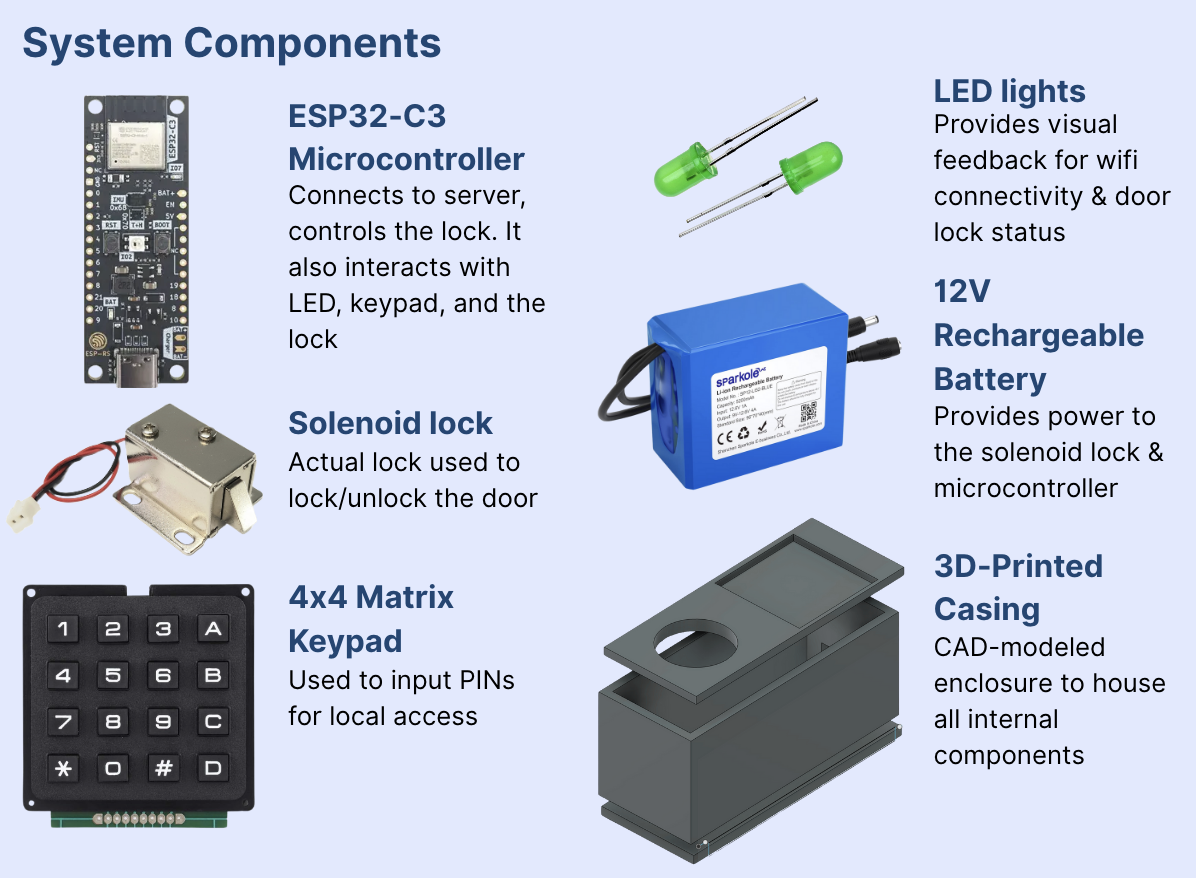
\includegraphics[width=1\textwidth]{img/hardwareComponents.png}
    \label{fig:hardwareComponents}
\end{figure}

For our hardware, we also used up 99\% of the ESP32-C3 storage. We also utilized power supplies for our functional prototype since the solenoid lock required 12V to unlock the lock. 

\subsection{Software}

The functional prototype of the app currently uses the Swift language. This is what we wanted especially for native IOS apps, and in our manufactured design we plan to use the same language. Though we also would like to produce the same app on other non IOS devices as well. The app currently is able to allow users to sign in and sign up, unlock and lock the door, generating one time pins, accessing emergency pins, and logging out. 

\begin{figure}[!ht]
    \centering
    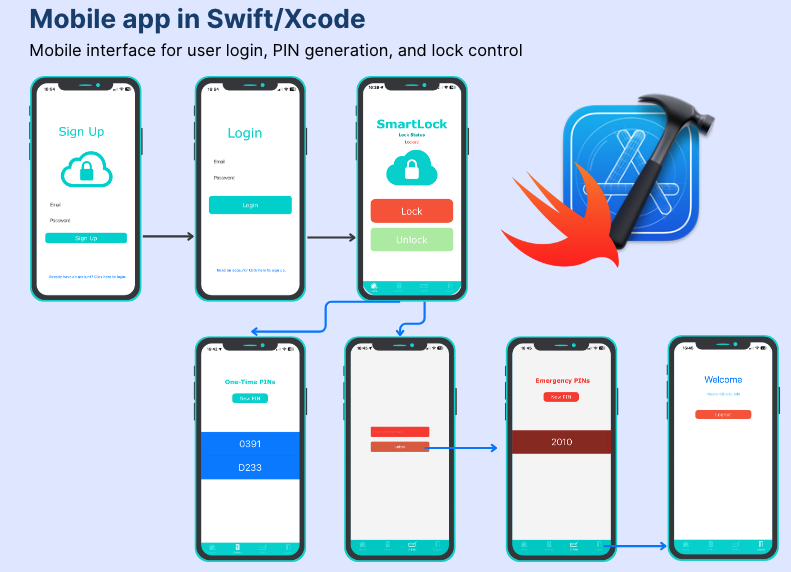
\includegraphics[width=1\textwidth]{img/softwareComponents.png}
    \label{fig:softwareComponents}
\end{figure}

\subsection{Cloud infrastructure}

Our current cloud infrastructure uses firestore database from firebase. Firebase was the easiest to use for our prototyping, and allowed us to quickly made the project functional. Though for the production system, we plan to use Amazon Web Services (AWS) along side Postgres so that we have more control on our database.  The current structure of our database only have a user controlling a lock, while we plan to update our cloud structure to have a many-to-many relationship. It should have a table for users and another table for locks, this way we can create a join table to join which users owns which lock and the lock is also able to know who the owner is. This is the common way people use the cloud structure to solve the many-to-many relationship.

\subsection{Results}

Our functional prototype was able to unlock and lock a door when asked to from the phone app. It can also generate pin codes that is for one time use, and the pin will be removed once the pin is used. Lastly we have an emergency pin that is used when the wifi is down. Once the emergency pin is used and the door lock is reconnected to wifi, it will remove the pin that is used. Compared to our manufactured product, we have a pin code to unlock the door but we did not have the feature of adding in how long the pin code lasts (having expiration on codes). As for the setup of the door lock, we used wifi provisioning instead of bluetooth since it seemed easier to create on ESP32-C3. Below we will have a figure of our final prototype and if you would like to see the demo of our prototype, the link is \href{https://youtu.be/XbD7zrFxasE?si=83Vg6o0KJSXbOtdF}{here}.

\begin{figure}[!ht]
\centering
\begin{subfigure}{.5\textwidth}
  \centering
  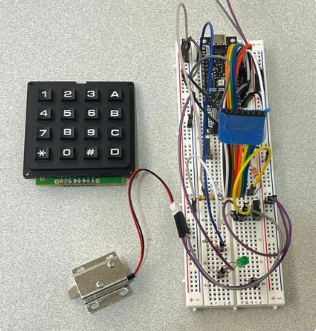
\includegraphics[width=.7\linewidth]{img/prototypeInside.png}
  \caption{inside of prototype}
  \label{fig:prototypeInside}
\end{subfigure}%
\begin{subfigure}{.5\textwidth}
  \centering
  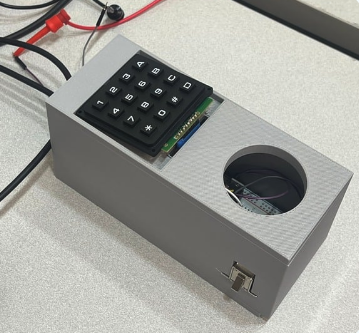
\includegraphics[width=.7\linewidth]{img/prototypeOutside.png}
  \caption{outside of prototype}
  \label{fig:prototypeOutside}
\end{subfigure}
\caption{Functional prototype result}
\label{fig:test}
\end{figure}